\chapter{Results}
\label{sec:results}
\lhead{\emph{Chapter 4. Results}}  % page header

This chapter reports the results in the order of the research questions: the field (Section~\ref{sec:field}), entry to
topics (Section~\ref{sec:entry}) and the acceptance decision (Section~\ref{sec:gate}). Table~\ref{tab:verdicts} first
gives the outcome of every registered hypothesis. The findings are listed together in Chapter~\ref{sec:conclusion}.

\begin{table}[tb]
\centering
\footnotesize
\setlength{\tabcolsep}{3pt}
\renewcommand{\arraystretch}{1.1}
\begin{tabularx}{\textwidth}{@{}l Y L{2.6cm} L{2.6cm} L{2.6cm}@{}}
\toprule
ID & Prediction & Discovery [95\% CI] & Held-out [95\% CI] & Outcome \\
\midrule
H1a & Method share falls as a topic grows & $-$0.14\newline[$-$1.8, +1.5] & -- & not supported \\
H1b & Measurement share rises & +0.50\newline[$-$0.8, +1.8] & -- & not supported \\
H1c & Empirical share rises & $-$0.31\newline[$-$1.3, +0.7] & -- & not supported \\
H1d & Fewer new architectures where FM adoption is high & $-$7.98\newline[$-$12.14, $-$3.82] & $-$11.0\newline[$-$18.1, $-$3.9]
& \lab{replicated} \\
H1e & More empirical or evaluation papers where FM adoption is high & $-$0.63\newline[$-$3.64, +2.38] & -- &
\lab{inconclusive} \\
\addlinespace
H2a & Entrants flock to hot topics & $-$0.73\newline[$-$2.68, +1.22] & -- & \lab{inconclusive} \\
H2b & Newcomers write fewer method papers & +3.71\newline[+2.61, +4.80] & +3.60\newline[+1.48, +5.71] & reversed;
\lab{replicated} \\
H2c & Newcomers write more measurement papers & $-$1.70\newline[$-$2.46, $-$0.93] & $-$2.10\newline[$-$3.35, $-$0.85] & reversed;
\lab{replicated} \\
\addlinespace
H3a & Crowded topics accepted less often & $-$1.68\newline[$-$3.68, +0.32] & $-$1.51\newline[$-$5.20, +2.19] &
\lab{uninformative} \\
H3b & Larger crowding penalty for method papers & $-$0.36\newline[$-$1.51, +0.79] & -- & not supported \\
\bottomrule
\end{tabularx}
\caption[Outcomes of the registered hypotheses]{Outcomes of the registered hypotheses (Table~\ref{tab:registered}).
Units are pp: per log unit of earlier papers for H1a--c and H3a--b, and for a change in prior FM adoption from 0 to
100\% for H1d--e. For H2b and H2c the registered prediction failed in the opposite direction; the reversed
hypotheses were registered before the held-out data were examined and were supported on held-out papers. Held-out
tests are one-sided.}
\label{tab:verdicts}
\end{table}

% ===============================================================================================================
\section{The field: what is a wave and what lasts (RQ1)}
\label{sec:field}

This section asks which changes in the field are passing waves and which persist.

\begin{figure}[tb]
  \centering
  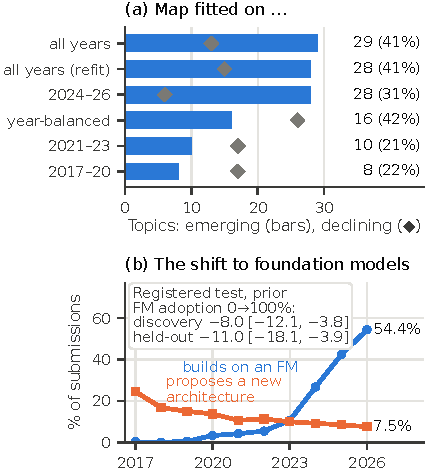
\includegraphics[width=0.62\textwidth]{figs/fig2_field.pdf}
  \caption[Emerging topics by fitting window, and the shift to foundation models]{(a) Emerging (bars) and declining
  (grey diamonds) topics on topic maps fitted on different years, for the same 43,480 papers. Labels at right show the
  number of emerging topics and, in brackets, the share of 2024--2026 papers in them (22.3\% on the 2017--2020 map,
  40.9\% on the all-years map); `all years (refit)' uses another random seed. Topic size `predicts' two-year growth
  only on the all-years map (out-of-sample $R^2 = 0.28$ against $-$0.03; no paired test). (b) Share of submissions
  building on an FM (blue) and proposing a new architecture (orange), using contribution types assigned by the LLM,
  with the registered test inset (\lab{replicated}).}
  \label{fig:field}
\end{figure}

\subsection{Waves}
Author keywords need no topic map, and at their level waves are real: 17 of the 68 most frequent keywords are
\emph{waves}, which rose and fell, peaking in 2019--2024 with shares of at most half the peak both before it and in
2026 (Figure~\ref{fig:waves}; \lab{exploratory}).

\subsection{Emergence depends on hindsight}
A topic is called \emph{emerging} if its 2024--2026 share is at least three times its 2017--2020 share, and
\emph{declining} if its 2024--2026 share is at most a third of its 2017--2020 share. With the same papers and pipeline,
a map fitted on 2017--2020 finds 8 emerging topics and one fitted on all years finds 29 (Figure~\ref{fig:field}a;
\lab{exploratory}). Two causes combine, and they cannot be separated. The all-years map uses the future to describe the
past, like leakage in prediction \citep{kapoor2023leakage} and hindsight bias in judgement
\citep{fischhoff1975hindsight}: with 69\% of its papers in 2024--2026, it is in effect a present-day map. The early map,
for its part, cannot represent topics born after 2020. The two counts therefore bracket the number of emerging topics.

The registered tests of whether a topic's contribution mix changes as it grows (H1a--c) were not supported on the
all-years map (Table~\ref{tab:verdicts}). On the early map, the method and measurement estimates point the predicted
way, so whether topics show such a life cycle also depends on how topics are defined.

\subsection{What lasts: the shift to foundation models}
The FM share rose every year from 2018 (Figure~\ref{fig:field}b). Prior FM adoption is associated with fewer
new-architecture papers (H1d): from 0 to 100\% adoption the difference is $-$7.98\,pp [$-$12.14, $-$3.82] in discovery
and $-$11.0 [$-$18.1, $-$3.9] on held-out papers (\lab{replicated}). The association may also run the other way. The
test for a parallel shift towards empirical or evaluation papers (H1e) is inconclusive ($-$0.63 [$-$3.64, +2.38]). The
pattern matches accounts of NLP's paradigm shifts \citep{gururaja2023build,saphra2024first,pramanick2023diachronic},
but lock-in \citep{hooker2021hardware}, efficient choice \citep{sutton2019bitter} and a bandwagon
\citep{fujimura1988molecular} predict it too. The field level therefore cannot separate the two routes.

% ===============================================================================================================
\section{Entry: who writes what (RQ2)}
\label{sec:entry}

This section asks what researchers write when they enter a topic, and whether they follow others into it as the
herding account implies.

\subsection{Newcomers propose methods}
The registered prediction was that newcomer papers, whose authors face the most uncertainty, would more often be
follow-on work: measurement papers that benchmark, collect data for or evaluate what others had proposed (H2b, H2c).
Newcomer papers make up 73\% of the 42,325 papers in 2019--2026 that have an author identifier. Compared with incumbent
papers, the difference in the share of method papers is +3.71\,pp [+2.61, +4.80] in discovery and +3.60 [+1.48, +5.71]
on held-out papers; for measurement papers it is $-$1.70 [$-$2.46, $-$0.93] and $-$2.10 [$-$3.35, $-$0.85]
(Table~\ref{tab:entry}, Figure~\ref{fig:entry}). Both contrasts are \lab{replicated}. The registered prediction thus
failed in the opposite direction, and the reversed hypotheses, registered before the held-out data were examined, were
supported on the held-out papers. All ten counted variants agree in sign, and the $t$-statistics (6.7 and $-$4.4) are
too large to be explained by the inflated false-positive rate reported in Section~\ref{sec:threats}. Team size accounts
for much of the measurement gap: with log team size as a control, the gap shrinks to $-$0.54 [$-$1.11, +0.04] in
discovery and $-$0.98 ($p = 0.10$) on held-out papers, whereas the method gap barely changes (+3.92 and +3.64).

\begin{table}[tb]
\centering
\footnotesize
\setlength{\tabcolsep}{3pt}
\renewcommand{\arraystretch}{1.1}
\begin{tabularx}{\textwidth}{@{}Y L{2.7cm} L{2.7cm} L{2.4cm}@{}}
\toprule
Contrast & Discovery [95\% CI] & Held-out [95\% CI] & Label \\
\midrule
Method paper & +3.71\newline[+2.61, +4.80] & +3.60\newline[+1.48, +5.71] & \lab{replicated} \\
Measurement paper & $-$1.70\newline[$-$2.46, $-$0.93] & $-$2.10\newline[$-$3.35, $-$0.85] & \lab{replicated} \\
Measurement paper, with log team size$^a$ & $-$0.54\newline[$-$1.11, +0.04] & $-$0.98\newline($p = 0.10$) &
\lab{registered variant} \\
\addlinespace
Method: returning topic newcomer $-$ incumbent$^b$ & +3.43\newline[+2.31, +4.55] & -- & \lab{exploratory} \\
Method: first-time team $-$ returning topic newcomer$^b$ & +0.92\newline[$-$0.44, +2.29] & -- & \lab{exploratory} \\
Distance from earlier ICLR work, own work excluded (percentile points) & +4.33\newline[+3.44, +5.22] & -- &
\lab{exploratory} \\
\addlinespace
Entry into hot topics: incumbent share, hot $-$ other topics$^c$ & $-$0.73\newline[$-$2.68, +1.22] & -- &
\lab{inconclusive} \\
\bottomrule
\end{tabularx}
\caption[Entry contrasts between newcomer and incumbent papers]{Entry contrasts: newcomer minus incumbent papers
unless the row names other profiles, in pp within topic and year. Held-out tests are one-sided. $^a$Registered
supplementary variant, outside the support rule. $^b$First-time team: no author has any earlier ICLR submission;
returning topic newcomer: an author has one, in another topic. $^c$H2a; no held-out test was registered.}
\label{tab:entry}
\end{table}

\subsection{Topic newcomers and first-time ICLR teams}
Newcomer papers split into those from first-time teams (26.3\% of papers; median team size 3) and those from returning
topic newcomers (46.7\%; median 5); incumbent papers make up the remaining 27.0\% (median 5). Returning topic newcomers
write method papers more often than incumbents (+3.43\,pp [+2.31, +4.55]) at the same median team size, and the
difference holds with team size controlled (+3.62). For first-time teams the difference is +4.35 [+2.82, +5.89], and
the interval for the gap between the two newcomer profiles includes zero (+0.92 [$-$0.44, +2.29]). All three contrasts
are \lab{exploratory}. The method surplus is therefore associated mainly with entering a topic, not with being new to
ICLR or with working in a small team, and it appears in every period, including before 2023.

The measurement gap behaves differently. For first-time teams it is accounted for by team size ($-$2.24 [$-$3.24,
$-$1.25] against incumbents, and +0.09 [$-$0.63, +0.80] with team size controlled); for returning topic newcomers part
of it remains ($-$1.47, and $-$0.81 [$-$1.46, $-$0.16] with team size controlled). The gap appears only in 2024--2026
(first-time teams against incumbents: $-$2.75 [$-$4.07, $-$1.44]). In the FM era, then, measurement papers are
concentrated among topic incumbents and larger teams. Team size is the only resource observed here; others, such as
compute, may also matter. NLP shows a parallel at the level of research trends, where tasks and methods lead and
datasets follow \citep{pramanick2023diachronic}.

\begin{figure}[tb]
  \centering
  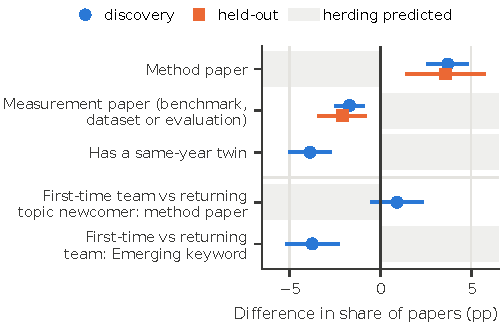
\includegraphics[width=0.72\textwidth]{figs/fig3_entry.pdf}
  \caption[Entry contrasts within topic and year]{Entry contrasts within topic and year (pp), with 95\% intervals:
  discovery (blue circles) and held-out (orange squares). Rows 1--2 compare newcomer with incumbent papers; they are
  registered and \lab{replicated}. Rows 3--5 are \lab{exploratory} (discovery only). Row 3 compares papers by returning
  topic newcomers with incumbent papers, with first-time teams entered separately and with contribution-type, FM and
  team-size controls. Row 4 compares first-time teams with returning topic newcomers, and row 5 compares first-time
  teams with returning teams (all teams with earlier ICLR submissions) on the use of young, rising Emerging keywords.
  Grey shading marks the side that the herding prediction expected.}
  \label{fig:entry}
\end{figure}

\subsection{Farther from earlier work}
Newcomer papers lie farther from earlier ICLR work than incumbent papers. Within topic and year the difference is
+5.90 percentile points [+4.95, +6.85]; it is +5.24 among method papers alone and +4.33 [+3.44, +5.22] when the
authors' own earlier papers are excluded from the reference set. Papers by returning topic newcomers are less likely
than incumbent papers to have a same-year \emph{twin}, an independent submission at cosine similarity $\geq 0.70$; with
first-time teams controlled separately, the difference in twin share is $-$3.86\,pp [$-$4.98, $-$2.74]. These results
are \lab{exploratory}. The follow-on prediction expects newcomer papers to lie closer to earlier work. Writing method
papers could itself be imitation of the venue's usual kind of paper, since three quarters of ICLR papers are method
papers, but newcomers' distance from earlier work argues against that reading. Neither contribution type nor embedding
distance measures originality; these results argue against newcomers following others but say nothing about whether
their work is more original.

\subsection{Later uptake of foundation models}
Among 2023--2026 papers in topics where 5--50\% of the previous year's papers built on FMs, the gap in FM-paper share
between first-time teams and returning topic newcomers is $-$4.58\,pp [$-$6.55, $-$2.60], widening to $-$14.71
[$-$19.82, $-$9.61] as adoption rises. For returning topic newcomers and incumbents the data show no clear difference.
First-time teams also list \emph{Emerging} keywords, which are young and rising, at a lower rate than teams with earlier
ICLR submissions; the difference is $-$3.74 [$-$5.14, $-$2.35]. Both results are \lab{exploratory}. Foundation models
thus spread through teams with earlier ICLR work, as absorptive capacity predicts \citep{cohen1990absorptive}. Network
diffusion predicts the same order, however, so this contrast cannot tell the routes apart.

\subsection{Flocking to hot topics}
Whether entrants crowd into hot topics remains open. The registered test (H2a), which compares the incumbent share in
hot and other topics, is inconclusive ($-$0.73 [$-$2.68, +1.22]), and no held-out test was registered for it. None of
the entry contrasts measured here favours the follow-on prediction.

% ===============================================================================================================
\section{The gate: crowd or record? (RQ3)}
\label{sec:gate}

This section asks whether acceptance at ICLR is associated with following the crowd or with staying close to the
authors' own earlier work. Table~\ref{tab:gate} and Figure~\ref{fig:gate} collect the tests. Of those in the figure,
crowding was registered, title style had been explored before registration and the remaining tests were found post hoc
in discovery; each held-out test was declared before any held-out estimate for its question was computed.

\subsection{Is following the crowd associated with acceptance?}
The registered crowding test (H3a) predicted a penalty for crowded topics, and it is uninformative. Per log unit of
crowding (the natural log of one plus the number of the topic's earlier papers), acceptance changes by $-$1.68\,pp
[$-$3.68, +0.32] in discovery and by $-$1.51 [$-$5.20, +2.19] on held-out papers, against an MDE80 of 4.8. The data
show no clear penalty or premium, although held-out premiums above +2.19\,pp per log unit lie outside the interval.
Whether the penalty is larger for method papers (H3b) could not be told ($-$0.36 [$-$1.51, +0.79]).

The clearest sign of imitation in the corpus is in title style. The share of titles that open with a short coined
name and a colon rose from 10.9\% in 2017 to 44.6\% in 2026. Within topic and year, with contribution-type, FM and
team-size controls, such branded titles are accepted 1.74\,pp [+0.37, +3.11] more often in discovery, but this estimate
is not a test, since title style had been explored before registration. The declared held-out test gives +1.76
[$-$0.82, +4.34] (one-sided $p = 0.089$); the held-out test is uninformative (below its MDE80 of 3.2), so the premium
remains \lab{exploratory}. Raw within-year gaps are larger (+3.3 in discovery and +4.0 on held-out papers); about half
of each gap is explained by topic, contribution type, FM use and team size. Titles can also be revised after the
decision, which could create such a premium.

FM papers are accepted 4.62\,pp more often [+2.79, +6.44], with no sign of a difference between late and early
adopters: the premium changes by +0.19 [$-$0.96, +1.34] per logit unit of the topic's prior FM adoption (that is, per
unit of its log-odds). Both results are \lab{exploratory}, and they fit efficient choice as well as imitation, if
review rewards it. A topic's \emph{edge} is its acceptance rate minus that of all other papers of the same year, using
topics of the 2017--2020 map. The edge persists but shrinks towards the mean: among discovery papers, the 2018--2022
edge predicts the 2024--2026 edge with slope 0.38 [0.18, 0.58]. The held-out test asks a related but different
question, namely whether the discovery edges for 2018--2022 predict the 2024--2026 edges of held-out papers; it gives a
slope of 0.60 [0.32, 0.88] and is \lab{held-out supported}. A favoured topic thus keeps only part of its edge, as
expected when decisions carry a large arbitrary component \citep{cortes2021inconsistency,beygelzimer2023has}.

Keyword timing shows at most weak associations, and it is treated as \lab{exploratory}: keyword popularity had been
explored against acceptance before registration, and both held-out intervals below include zero. On held-out papers,
\emph{Emerging} keywords (young and rising) are associated with higher acceptance than \emph{Mainstream} keywords (old
and flat), by +3.25 [$-$0.18, +6.69], and acceptance may fall after a keyword's share peaks ($-$5.2 [$-$11.1, +0.7];
$-$1.7 without the six keywords examined before this test was declared). Neither pattern shows the constant premium for
popular keywords that imitation would predict if review rewarded it.

\begin{table}[tb]
\centering
\footnotesize
\setlength{\tabcolsep}{3pt}
\renewcommand{\arraystretch}{1.1}
\begin{tabularx}{\textwidth}{@{}Y L{2.7cm} L{2.7cm} L{2.4cm}@{}}
\toprule
Contrast in acceptance & Discovery [95\% CI] & Held-out [95\% CI] & Label \\
\midrule
\multicolumn{4}{@{}l}{\textit{Referenced to the team's own record}} \\
Far jump: 10th percentile of \Fmax{} $-$ median & $-$5.44\newline[$-$7.10, $-$3.78] & $-$6.09\newline[$-$9.32,
$-$2.86] & \lab{held-out supported} \\
Same author, 0.1 closer in cosine similarity$^c$ & +0.55\newline[+0.21, +0.90] & +1.06\newline[+0.23, +1.89] &
\lab{held-out supported} \\
One topic insider vs none$^c$ & +3.42\newline[+1.18, +5.66] & +3.88\newline[+0.28, +7.47] & \lab{held-out supported} \\
\addlinespace
\multicolumn{4}{@{}l}{\textit{Referenced to others or the field}} \\
Crowding, per log unit$^a$ & $-$1.68\newline[$-$3.68, +0.32] & $-$1.51\newline[$-$5.20, +2.19] & \lab{uninformative} \\
Branded title$^b$ & +1.74\newline[+0.37, +3.11] & +1.76\newline[$-$0.82, +4.34] & \lab{exploratory} \\
Change in FM premium per logit unit of prior adoption & +0.19\newline[$-$0.96, +1.34] & -- & \lab{exploratory} \\
Topic edge 2018--22 \ra{} 2024--26, slope$^c$ & 0.38\newline[0.18, 0.58] & 0.60\newline[0.32, 0.88] & \lab{held-out
supported} \\
Emerging $-$ Mainstream keyword$^{b,c}$ & +2.67\newline[+0.76, +4.58] & +3.25\newline[$-$0.18, +6.69] &
\lab{exploratory} \\
Distance from earlier ICLR work: least-distant fifth $-$ middle fifth & $-$3.27\newline[$-$4.93, $-$1.60] &
$-$0.13\newline[$-$3.50, +3.25] & \lab{uninformative} \\
\bottomrule
\end{tabularx}
\caption[Acceptance contrasts at the gate]{Acceptance contrasts at the gate, in pp within topic and year (topic edges
and keywords: against the same year's other papers). Rows differ in population and unit, so their sizes are not
comparable. Held-out tests are one-sided. $^a$Registered (H3a); predicted a penalty; MDE80 4.8. $^b$Explored against
acceptance before registration. For titles the discovery estimate is not a test (held-out MDE80 3.2); for keywords it
is a declared post hoc test on a dimension already seen. $^c$Holm-adjusted $p$ across the six secondary held-out tests:
topic-edge slope 0.019, edge prediction 0.026, same-author closeness 0.026, insider 0.052, Emerging keywords 0.063,
same-author distance slope 0.22.}
\label{tab:gate}
\end{table}

\begin{figure}[tb]
  \centering
  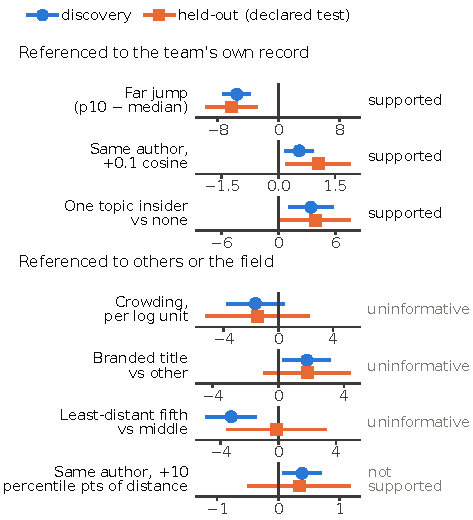
\includegraphics[width=0.72\textwidth]{figs/fig4_gate.pdf}
  \caption[Gate tests by reference point]{Gate tests by reference point: discovery estimates (blue circles) and
  declared held-out tests (orange squares), with 95\% intervals. The held-out verdict is shown at right: `supported' means
  \lab{held-out supported}; `uninformative' means not supported and below the test's MDE80; `not supported' marks a
  declared test without a registered MDE80, which is called inconclusive in the text. Each row has its own scale: pp for
  the far jump (closeness at its 10th percentile, p10, minus the median), the insider, the branded title and the
  least-distant fifth; pp per log unit for crowding; and pp per 0.1 cosine similarity and per 10 percentile points of
  distance for the two same-author slopes. Because the scales differ, compare verdicts rather than sizes.}
  \label{fig:gate}
\end{figure}

\subsection{What is acceptance associated with?}
The main pattern is the \emph{far jump}: the lower acceptance of papers far from the team's earlier work. Among
20,430 decided 2023--2026 papers with an experienced author, acceptance at the 10th percentile of closeness to the
team's own record is 5.44\,pp lower than at the median in discovery ($-$5.44 [$-$7.10, $-$3.78]) and 6.09\,pp lower on
held-out papers ($-$6.09 [$-$9.32, $-$2.86]), with power = 0.89. This was the primary test declared for the held-out
papers, and it is \lab{held-out supported}. Adjusted acceptance rises with closeness up to the fourth fifth of the
distribution. The far jump remains with a newcomer control ($-$5.0), although closeness is correlated with newcomer
status ($r = -0.57$).

Holding the author fixed, a paper 0.1 closer in cosine similarity to that author's earlier work is associated with
acceptance 0.55\,pp higher [+0.21, +0.90] in discovery and 1.06\,pp higher [+0.23, +1.89] on held-out papers. This
result is \lab{held-out supported} and survives a family-wise correction across the secondary tests. Controls for
newcomer status and for co-authors' experience change it little (+0.48 and +0.50), though unmeasured differences in
co-author quality could also bias it; a simulation run before the held-out test showed that such a confounder can
shift the estimate. In a related within-author comparison, on a paper in a topic new to them, the same author's
acceptance is 1.37\,pp lower ($-$1.37 [$-$2.74, $-$0.004]; author fixed effects, \lab{exploratory}).\footnote{Newcomer
papers as a whole have 10.2\,pp lower acceptance ($-$10.2 [$-$11.8, $-$8.7]) within topic and year
(\lab{exploratory}), but that gap mostly reflects who writes them: it shrinks once team size and the authors' ICLR
experience are controlled, and shrinks further within the same authors.}

Having one topic insider on the team, rather than none, is associated with acceptance 3.42\,pp higher [+1.18, +5.66] in
discovery and 3.88\,pp higher [+0.28, +7.47] on held-out papers, at fixed team size and number of experienced authors
(\lab{held-out supported}). The result does not survive the family-wise correction (Holm-adjusted $p = 0.052$), and
status explains it equally well: each additional insider adds only 0.58\,pp more than each additional experienced
author from another topic ($p = 0.16$; \lab{exploratory}).

Distance from earlier ICLR work as a whole gives uninformative results. In the same SPECTER2 vector space, papers in
the least-distant fifth differ from those in the middle fifth by $-$3.27 [$-$4.93, $-$1.60] in discovery but by $-$0.13
[$-$3.50, +3.25] on held-out papers, a test with power = 0.47. The within-author slope for distance from earlier ICLR
work was not supported either, and with no MDE80 available it is inconclusive. Of the distance-based tests, only the
associations with the team's own earlier work held up on held-out papers.
